\chapter{Einleitung}

\section{Die Aufgabenstellung}

Im Rahmen der Aufgabenstellung zum Kurs "DLMDWPMP01 – Programmieren mit Python" soll ein Python-Programm umgesetzt werden, das "verwaschene" Trainingsdaten korrekt auf vier idealtypische Funktionen abbildet. Hierfür stehen 50 idealtypische Funktionen zur Auswahl. Maßgeblich für die Auswahl ist hierbei, gemäß Vorgabe, die kleinste Summe der quadratischen Abweichungen (Least-Square).
Anschließend soll das gleiche Programm die Punkte eines Testdatensatzes, anhand eines definierten minimalen, statistischen Abstandswertes zu den gewählten idealtypischen Funktionen, klassifizieren und jeweils der entsprechenden Funktion zuordnen.
Fokus der vorliegenden Aufgabenstellung, sowie dieser Arbeit war jedoch primär die Erlernung der Programmiersprache Python und nicht die ausschließliche Erfüllung der beschriebenen mathematischen Aspekte. Diese, isoliert betrachtet, hätte ebenso in Form eines einfachen Jupyter-Notebooks erarbeitet werden können.


\section{Installationshinweise}

Das Programm wurde vom Autor mit dem Namen \emph{"functionfinder"} betitelt und steht auf GitHub unter dem Link \begin{center}\url{https://github.com/GGProjects/DLMDWPMP01}\end{center} zum Download zur Verfügung.

In der folgenden Abbildung werden die wesentlichen Elemente der bereitgestellten Modulstruktur dargestellt. Hervorzuheben ist hierbei das Verzeichnis \emph{functionfinder}, welches jene Pythondateien beinhaltet, die für die Programmfunktionalität verantwortlich sind.
Die übrigen Verzeichnisse stehen für die bereitgestellten Daten (\emph{data}), die vom Programm erzeugten Ausgaben (\emph{output}), sowie für die vorgesehenen UnitTests (\emph{tests}) zur Verfügung.

\definecolor{mygray}{rgb}{0.9,0.9,0.9}
\lstset{backgroundcolor=\color{mygray},
	captionpos=b,  % sets the caption-position to bottom
	emph={functionfinder}, 
	emphstyle=\color{red},
	basicstyle=\small,
	frame=single,
	framextopmargin=6pt,
	framexbottommargin=6pt,
	morecomment=[l][\color{red}]{/},}
	
\begin{tabular}{c}  % the tabular makes the listing as small as possible and centers it
\lstinputlisting[caption={Struktur des Moduls},
	label=folder]{tree.txt}
\end{tabular}


Für die Installation bietet es sich an, lokal eine virtuelle Pythonumgebung anzulegen. Anschließend kann nach Wechsel in das Modulverzeichnis, mit dem Befehl
\begin{center}\emph{pip install -e .}\end{center}
die Datei \emph{setup.py} ausgeführt und somit das Modul installiert werden.
Mit der Installation wird die Verfügbarkeit der benötigten Dateien überprüft und UnitTests zur Sicherstellung der Funktionalität durchgeführt. Benötigte Pakete werden gegebenenfalls in der virtuellen Umgebung nachinstalliert. Im Rahmen der Installation wird außerdem ein Logfile mit der Bezeichnung \emph{setuplog\_[DATUM]\_[UHRZEIT]} im Verzeichnis \emph{output/logs} angelegt.
Nach erfolgreicher Installation, kann das Programm aus der Konsole mit dem einfachen Aufruf \emph{ff} ausgeführt werden.
Im Zuge der Entwicklung wurde das vorliegende Programm mit der Pythonversion 3.11 unter Windows10 getestet.

\section{Konfigurationshinweise}

Über Änderungen in der Datei \emph{functionfinder/config.py} können, falls benötigt, Verzeichnispfade, Log-Einstellungen, Bewertungsfunktionen, sowie auch die Pfade zu den vorliegenden Datendateien angepasst werden.

Letzteres ermöglicht eine einfache Änderung der verwendeten Trainings-, Funktions- und Testdaten, um das Programm auch mit anderen als den, im Rahmen der Aufgabenstellung, bereitgestellten Daten auszuführen.

Eine Anpassung der Bewertungsfunktionen bietet des weiteren die Möglichkeit, die zur Bewertung der Trainingsdaten herangezogene Funktion (der Standardwert ist hierfür die kleinste Summe der quadratischen Abweichungen) sowie den Faktor für den errechneten Fehlerwert, zur Klassifikation der Testdaten (der Standardwert ist, gemäß Aufgabenstellung, die Wurzel aus Zwei) zu verändern.

\section{Struktur der Hausarbeit}

Im Hauptteil der vorliegenden Hausarbeit wird zuerst auf die bereitgestellten Datensätze eingegangen und wie diese, im Rahmen der Aufgabenstellung, verarbeitet wurden.
Anschließend wird in einem weiteren Unterkapitel die Auswahl an idealtypischen Funktionen anhand der vorliegenden Trainingsdaten beschrieben und dargestellt.
Das dritte Unterkapitel diskutiert die Klassifikation der Testdaten mithilfe der ausgewählten idealtypischen Funktionen. Hierbei wird auch auf die automatisierte Ausgabe zur Evaluierung nicht erfolgreich klassifizierter Testdaten eingegangen.
In der Zusammenfassung werden, anhand der dargestellten Ergebnisse, mögliche Anpassungen des Programms zur Verarbeitung größerer Datenmengen angesprochen und als potentielles Thema für eine weitere Hausarbeit zur Diskussion gestellt.

\chapter{Hauptteil}

\section{Bereitgestellte Datensätze}

Im Zuge der Aufgabenstellung wurden, zur Bearbeitung dieser, drei Datensätze angefertigt und in Form unten aufgelisteter CSV-Dateien bereitgestellt.

\begin{itemize}
 \itemsep0pt
 \item \emph{train.csv}
 \item \emph{ideal.csv}
 \item \emph{test.csv}
\end{itemize}

Erstere beinhaltet eine Tabelle von vier "verwaschenen" Funktionen in den Spalten \emph{y1} bis \emph{y4} mit jeweils 400 Datenpunkten. Die folgende Tabelle zeigt die exemplarische Struktur des Trainingsdatensatzes.

\begin{table}[H]
\small
\centering
\csvautotabular[range={+5}]{../data/train.csv}
\caption{Exemplarischer Auszug der Datei train.csv}
\label{tab:Exemplarischer Auszug aus train.csv}
\end{table} 


Eine Visualisierung der Trainingsdaten lässt bereits optische Rückschlüsse auf passende idealtypische Funktionen zu.
\begin{figure}[h]
\centering
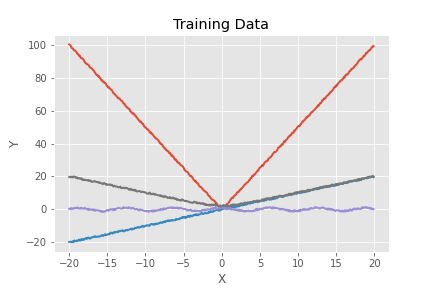
\includegraphics[width=12cm]{../output/figures/train.png}
\caption{Darstellung der bereitgestellten Trainingsdatensätze \cite{Gage:18}}\label{fig:train}
\end{figure}

Die Datei ideal.csv beinhaltet 50, nicht "verwaschene", idealtypische Funktionen in den Spalten \emph{y1} bis \emph{y50}. Wie im Detail im folgenden Unterkapitel beschrieben, sollen diese Funktionen durch das Programm mit dem Trainingsdatensatz verglichen werden und daraus die passendsten vier Funktionen gewählt werden. Die Datei weist, bis auf die Anzahl der Spalten, eine ähnliche Struktur wie der Trainingsdatensatz auf und besteht ebenfalls je Spalte aus 400 Datenpunkten. Auf die Darstellung eines exemplarischen Auszuges wird daher an dieser Stelle verzichtet.

\begin{table}[H]
\small
\centering
\csvreader[
	tabular = ccccc,
	range={+5},
	late after line = \\\hline,
	no head]%
  {../data/ideal.csv}{}{%
  \csvcoli & \csvcolii & \csvcoliii & \csvcoll & \csvcolli}
%\csvautotabular[range={+5}]{../data/ideal.csv}{}{\csvcoli & \csvcolii & \csvcoliii & \csvcoll & %\csvcolli}
\caption{Exemplarischer Auszug der Datei ideal.csv}
\label{tab:Exemplarischer Auszug aus ideal.csv}
\end{table} 

Im Gegenzug zu den oben dargestellten beiden Datensätzen besteht der Testdatensatz nur aus 100 einzelnen Datenpunkten. Diese werden in einer Spalte \emph{y} der Datei \emph{test.csv} zusammengefasst und sind nicht als zusammengehörige Funktion zu verstehen. 

\begin{table}[H]
\small
\centering
\csvautotabular[range={+5}]{../data/test.csv}
\caption{Exemplarischer Auszug der Datei test.csv}
\label{tab:Exemplarischer Auszug aus test.csv}
\end{table} 

In der weiteren Bearbeitung der Aufgabenstellung sollen diese Datenpunkte mit den ausgewählten idealtypischen Funktionen verglichen und jeweils jener mit der geringsten Abweichung zugewiesen werden. Dieser Vorgang wird im Zuge dieser Arbeit als Klassifikation der Testdaten bezeichnet. Diese wird im Unterkapitel "Klassifikation der Testdaten" im Detail behandelt.

Gemäß der Vorgabe der Aufgabenstellung sollen sowohl die Trainings- (\emph{train.csv}) als auch die Funktionsdaten (\emph{ideal.csv}) in eine SQLite Datenbank eingelesen werden. Diese wird im Verzeichnis \emph{output/data} bereitgestellt. Der Autor entschied sich hierbei für das Python-Modul \emph{sqlite3} anstelle des, in der Vorgabe vorgeschlagenen, Moduls \emph{sqlalchemy}. Dieses bietet für die gegebene Anwendung eine vereinfachte Möglichkeit Daten mit einer SQLite Datenbank zu verarbeiten.

Über die UnitTests, die im Rahmen der, in Kapitel 1.2 beschriebenen, Modulinstallation durchgeführt werden, wird das lokale System auf die Möglichkeit eines direkten SQL-Imports hin überprüft. Dies bedeutet, dass versucht wird, die Daten in die SQLite Datenbank zu schreiben, ohne diese zuerst über das Python-Programm einzulesen und erst in einem weiteren Verarbeitungsschritt an die Datenbank zu übergeben. Das Ergebnis der Überprüfung wird bei Erfolg im Logfile des Setups angeführt. 

Auch in der Ausführung des Programms wird vorerst noch einmal der direkte Import versucht und erst im Falle eines Fehlschlages der Umweg über die Funktionen des Python-Moduls \emph{pandas} gewählt.

Obwohl, aufgrund der geringen Größe, der in dieser Arbeit vorliegenden Datendateien, die Möglichkeit des direkten Imports nur eine untergeordnete Rolle spielt, schont ein solcher im Falle von größeren Datenmengen die Systemressourcen und spart Zeit in der Programmausführung.

Die Testdaten (\emph{test.csv}) werden, gemäß Vorgabe, in der Programmausführung zeilenweise eingelesen, mit den Daten der gewählten Funktionen verglichen und gemeinsam mit der getroffenen Klassifikation in die SQLite Datenbank geschrieben.

Für die interne Verarbeitung der Daten wurde, im Rahmen des Programms, eine eigene Objektklasse geschaffen, die spezifische Funktionen sowie die Parameter der Visualisierung bereitstellt. Diese Klasse und deren Unterklassen für die verschiedenen Datensätze sind in der Datei \emph{functionfinder/classes.py} definiert.

\section{Auswahl idealtypischer Funktionen}

Wie bereits im vorangegangenen Unterkapitel angeführt, steht zur Bearbeitung der Aufgabenstellung eine Auswahl an 50 idealtypischen Funktionen in einer CSV-Datei zur Verfügung. Aus diesen sollen für jede der vier Datenspalten der Trainingsdaten jeweils die passendste Funktion durch das Programm gewählt werden. Das Kriterium zur Selektion ist, gemäß Aufgabenstellung, die Minimierung der Summe aller quadratischen y-Abweichungen (Least-Square).

Mathematisch wird daher der kleinste Wert der Formel
\begin{equation}  
\sum_{i=1}^{n}(TrainingData_{i} - IdealFunction_{i})^2
\label{leastsquare}
\end{equation}
gesucht. Wobei die Variable $TrainingData$ durch alle vier vorliegenden Trainingsdatenspalten iteriert und die Variable $IdealFunction$ durch sämtliche verfügbaren Datenspalten der idealtypischen Funktionen. $n$ steht hierbei für die Anzahl an Datenpunkten je Datenspalte, die in beiden Datensätzen gleichgroß sein muss. 

In der Ausführung des programmierten Moduls wurde für den mathematischen Teil dieser Aufgabe (gemäß Gleichung ~\ref{leastsquare})  von der Eigenschaft des \emph{pandas}-Objekts \emph{Series} Gebrauch gemacht, die, bei der Subtraktion von zwei gleichlangen \emph{Series} der Länge $n$ (in diesem Fall mit $n=400$) erneut eine \emph{Serie} derselben Länge mit den jeweils subtrahierten Einzelwerten zurück gibt. Auch die mathematische Funktion des Quadrats wird auf jeden Einzelwert der Serie angewandt. Die Summenbildung der Serie fasst diese nun, dem vorgegebenen Kriterium entsprechend, zu einem Wert zusammen.
Diese Eigenschaft ermöglichte es daher, jede Datenspalte des Trainingsdatensatzes durch die Datenspalten der verfügbaren idealtypischen Funktionen zu iterieren und die zurückgelieferten Ergebnisse direkt zu vergleichen. Das Ergebnis mit der kleinsten Summe wurde jeweils als das Passendste abgespeichert.

Im Programmdesign bot es sich daher an, hierfür zwei Methoden getrennt zu definieren:
\begin{enumerate}
 \itemsep0pt
 \item Die Methode der Iteration und des Vergleiches zur Ermittlung des minimalen Fehlers wurde im Modul \emph{functionfinder/datafunctions.py} definiert.
 \item Die Methode zur Berechnung des Fehlers (gemäß Vorgabe, entsprechend der Gleichung ~\ref{leastsquare}) wurde in der Datei \emph{functionfinder/config.py} definiert.
\end{enumerate}

Dies erlaubt es, auf einfache Weise in der Konfigurationsdatei \emph{functionfinder/config.py}, die Methode zur Fehlerberechnung zu verändern und gegebenenfalls andere Kriterien, wie zB die durchschnittliche mittlere Abweichung (Mean Squared Error - MSE) zur Bewertung heranzuziehen. 

Als Rückgabewert der ersten genannten Methode, wurde vom Autor der Python-Datentyp \emph{dictionary} gewählt. In diesem wurde zu jedem \emph{Key} (die Datenspalten des Trainingsdatensatzes) der \emph{Value} in Form eines \emph{Tupels} abgelegt, welcher den Namen der gewählten Datenspalte des Datensatzes idealtypischer Funktionen, sowie die berechnete Abweichung beinhaltet.

\begin{tabular}{c}  % the tabular makes the listing as small as possible and centers it
\begin{lstlisting}[language=python,
				   caption={Darstellung des Rückgabewertes der berechneten Übereinstimmungen},
				   label=dictresult]
{'y1': ('y36', 33.71178854422821),
 'y2': ('y11', 32.62893138832121),
 'y3': ('y2', 33.11847188090256),
 'y4': ('y33', 31.75243110139478)}
\end{lstlisting}
\end{tabular}

Die oben angeführte Darstellung des Rückgabewertes macht ersichtlich, welche idealtypischen Funktionen für die jeweiligen Trainingsdatenspalten gewählt wurden. Die grafische Repräsentation lässt auch eine optische Bestätigung der getroffenen Auswahl zu.

\begin{figure}[h]
\centering
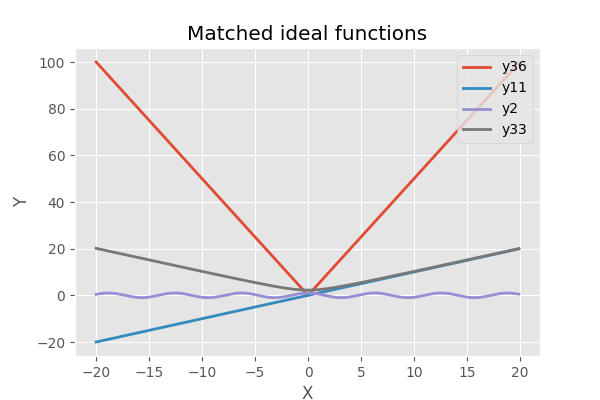
\includegraphics[width=12cm]{../output/figures/ideal.png}
\caption{Darstellung der ausgewählten idealtypischen Funktionen \cite{Gage:18}}
\label{fig:ideal}
\end{figure}

\section{Klassifikation der Testdaten}

In diesem Unterkapitel wird die Klassifikation der Testdaten mithilfe der ausgewählten idealtypischen Funktionen sowie den jeweiligen berechneten Abweichungen (siehe vorangegangenes Unterkapitel) diskutiert.

Entsprechend der Vorgabe zur vorliegenden Aufgabenstellung sollen die, in der Datei \emph{test.csv}, abgebildeten Datenpunkte, Zeile für Zeile eingelesen und mit dem maximalen Abstand von $ a*\sqrt{2}$ einer der vier gewählten Funktionen zuordnet. Wobei $a$ den berechneten Fehlerwert des Trainingsdatensatzes der jeweiligen Funktion repräsentiert.

In der Umsetzung wurde oben angeführte Berechnungsformel wiederum in zwei Teile zerlegt. Der Wert $a$ stammt aus einer vorangegangenen Berechnung und ist an dieser Stelle bereits bestimmt. Der zweite Teil betrifft den Multiplikationsfaktor $\sqrt{2}$, welcher durch die Vorgabe zur Aufgabenstellung festgelegt wurde. Um diesen gegebenenfalls anpassen zu können wurde dazu die Variable \emph{factor} in der Konfigruationsdatei \emph{functionfinder/config.py} definiert. Dadurch wird wiederum eine flexible Herangehensweise an die Bewertung der Testdaten gewährleistet.

Für die Bewertung selbst wurde in der Datei \emph{functionfinder/datafunctions.py} die Methode \emph{calculate\_best\_ideal} definiert. Diese nimmt im Wesentlichen als Parameter die aktuell eingelesene Zeile der Datei \emph{test.csv}, die Auswahl der idealtypischen Funktionen inklusive der Fehlerberechnungen, den Datensatz der idealtypischen Funktionen, sowie einen Funktionsparameter für die Filterung der Ergebnisse entgegen. 

Letzterer ist für die Berechnung der passenden idealtypischen Funktion auf \emph{min} gesetzt. Das bedeutet, dass aus den Abweichungen zu allen vier gewählten Funktionen, diejenige mit der kleinsten Abweichung gewählt wird.

Die Aufgabenstellung sieht vor, dass die Testdaten um die Werte der Abweichung (DeltaY), sowie die Nummer der gewählten Funktion (Idealfunktion) erweitert werden und in eine eigene Tabelle der SQLite Datenbank geschrieben werden. Der Autor entschied sich an dieser Stelle, noch einen Wert (Off\_limit) hinzuzufügen. Dieser Wert, vom Datentyp \emph{Boolean}, zeigt an, wenn dieser Datenpunkt den gesetzten Maximalabstand ($a*\sqrt{2}$) zu keiner der gewählten Funktionen einhalten konnte und wird in diesem Fall auf \emph{True} gesetzt. Dem Datenpunkt wird aber dennoch die Funktion mit dem geringsten Abstand zugewiesen.

Exemplarischer Auszug der Ergebnisse aus der SQLite Datenbank:



Für eine Evaluierung der Ergebnisse wurde in der Objektklasse \emph{testdata} die Methode \emph{off\_limit} definiert, die aus der SQLite Datenbank jene Werte abfragt, bei denen dieser Wert auf \emph{True} gesetzt ist. Diese Datenpunkte werden nochmals an die Methode \emph{calculate\_best\_ideal} übergeben, wobei diesmal der Funktionsparameter für die Filterung auf \emph{raw} gesetzt wird. Dadurch werden die Ergebnisse des Vergleichs zu jeder der vier gewählten idealtypischen Funktionen ausgegeben und können über das Logfile manuell evaluiert werden.

Bei der Bearbeitung der zur Aufgabe übergebenen Datensätze waren hierbei zwei Datenpunkte des Testdatensatzes betroffen. Der aufbereitete Auszug aus dem entsprechenden Logfile zeigt die unten angeführten Ergebnisse:

\begin{lstlisting}[caption={Datenpunkte mit überschrittenem Maximalabstand},
				   label=offlimit]
/  2 entries had a deviation above the set limit:

|  x         y     DeltaY Idealfunktion  Off_limit
/ -6.5  81.21402  48.714020           y36       True
| -6.5  81.21402  87.714020           y11       True
| -6.5  81.21402  80.237432            y2       True
| -6.5  81.21402  74.340156           y33       True

|  x         y     DeltaY Idealfunktion  Off_limit
| 0.3  59.68033  58.180330           y36       True
| 0.3  59.68033  59.380330           y11       True
| 0.3  59.68033  58.724993            y2       True
/ 0.3  59.68033  57.424227           y33       True
\end{lstlisting}

In den oben angeführten Tabellen wird die Distanz der beiden betroffenen Datenpunkte zu den vier gewählten Funktionen ersichtlich. In der Zuweisung wurden dennoch jene Funktionen mit dem geringsten Abstand gewählt (grafisch hervorgehoben).

In der grafischen Repräsentation der Ergebnisse ist die Annäherung der einzelnen Datenpunkte des Testdatensatzes an die gewählten idealtypischen Funktionen gut erkennbar. Jene beiden Datenpunkte, die im Vergleich den definierten Maximalabstand überschritten haben werden durch das Symbol $x$ dargestellt. Wobei hier die optische Beurteilung des zweiten Punktes eher eine Tendenz zur Funktion \emph{y36} vermuten ließe, als zur Funktion \emph{y33}. In der oben angeführten Tabelle zu diesem Datenpunkt wird aber auch deutlich, dass die Berechneten Abstände tatsächlich sehr nahe beieinander liegen.

Zusätzlich kann in der Visualisierung beobachtet werden, dass auch an den Schnittpunkten der Funktionen die Zuordnung der Datenpunkte ausreichend gut zu funktionieren scheint und der Verlauf der idealtypischen Funktionen optisch erkennbar nachverfolgt wird.


\begin{figure}[h]
\centering
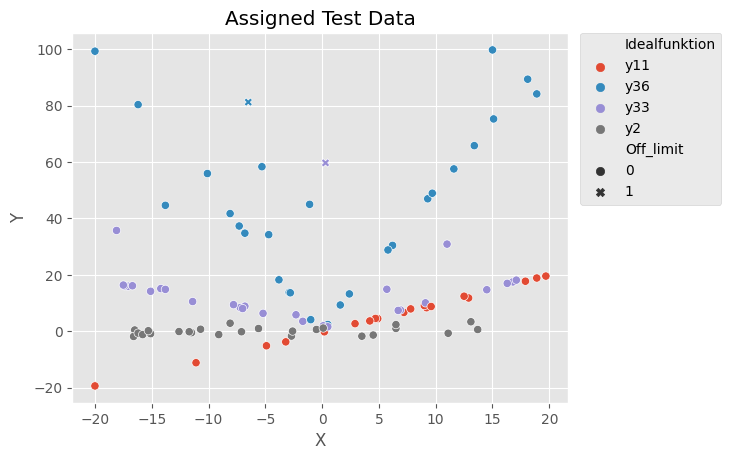
\includegraphics[width=12cm]{../output/figures/test.png}
\caption{Klassifikation der Testdatensätze \cite{Gage:18}}\label{fig:test}
\end{figure}


\chapter{Zusammenfassung}

Zeitersparnis: Tabellenweise verarbeitung der Testdaten
Zuweisung nicht aufgrund des kleinsten Abstandes sondern aufgrund des kleinsten Abstandes in Bezug auf $a$ (den berechneten Fehlerwert der Trainingsdaten)



% =========================================================
\section{Literature References}
Here is an example of a reference with a page-number: \cite[S. 6]{DueckKo:2016}


\section{Pictures}

\begin{figure}[h]
\centering

\includegraphics[width=8cm]{pics/spiral.pdf}
\caption{A spiral... smooth vector-based with a clean parametrisation! \\ Nothing to do with \cite{Gage:18}}\label{fig:spiral}
\end{figure}
\FloatBarrier

\section{Tables}

\begin{table}[H]
\small
\centering
\begin{tabular}{p{5cm}|l|p{3cm}}
`` Industrial era '' &  ``Jobs '' & `` Wanted: Upgrade''' \\ \hline
Parts exchanger & Fitter & mecatronics specialist \\
eShop & reseller & `` Client-suggester'' \\
`` Coding-guru''' & Softwaredesign & Whole-life designer \\
JA! Gut \& Günstig & brand-names & `` Life-Style Feeling'' \\
Internetbanking & Bank clerk & Customer adviser \\
Robots & Specialist & Machine supervisor \\
Bush & Gardener & Nature-sculptor \\
Painting & Painter & Interior Design \\
 &  & \\
\end{tabular}
\caption[Downgrade and upgrade of job denominations]{Downgrade and Upgrade of job denominations \\ \ \ \ \cite{DueckKo:2016}}
\label{tab:Downgrade and Upgrade of job denominations}
\end{table} 

\section{Listes}

\begin{itemize}
 \itemsep0pt
 \item one
 \item twoi
 \item threei
\end{itemize}

\begin{enumerate}
 \itemsep0pt
 \item first
 \item second
 \item third
\end{enumerate}


\section{Formulæ}

A formula can be written inline, e.g. as $ \frac{d}{dx}\mbox{arctg}(x) = \frac{1}{1+x^2}$ or, in centered math:

\begin{equation}  \frac{d}{dx}\mbox{arctg}(x) = \frac{1}{1+x^2} \label{arctanderivative}\end{equation}

Notice that formulæ that are centered start bigger (technically, they start in \verb+\displaystyle+) than they start inline (technically, they start in \verb+\textstyle+ all subsequents reductions, e.g. an exponent, goes to \verb+\scriptstyle+ then \verb+\scriptscriptstyle+). Indeed a best effort is made so that inline formulæ do not change the line height which would bother the eye of a reader.

Formulæ can be given a number and a label. Numbering happens automatically with \verb+\begin{equation}+ and \verb+\end{equation}+ and can be avoided if enclosing the formula betwee \verb+\[+ and \verb+\]+. If using the \verb+\label+ macro inside, you can refer automatically to this equation using \verb+\ref{label}+. E.g. Thanks to equation~\ref{arctanderivative} one dare say that:

\begin{equation} \int_0^t \frac{1}{1+x^2} dx = \mbox{arctan}(t) \end{equation}


\section{Tools and Code}

Many users of this template will want to include some code.

The simplest way to do so is to use the \verb+\verb+ macro which is followed by a sign, then some code, then the sign again to close. This is the inline version which works as in: 


\begin{verbatim}
As we could calculate with \cite{Wolfram_alpha} using 
\verb_integrate 1 / pi e ^ (t/pi) from zero to infinity_.
\end{verbatim}

which yields: 

As we could calculate with \cite{Wolfram_alpha} using \verb_integrate 1 / pi e ^ (t/pi)_ from zero to infinity.


The multiline version of this is called \verb+\begin{verbatim}+ and finishes with \verb+\end{verbatim}+.


\section{Citation examples}

Monography \citep[][S. 22]{con:infra} 

Collection \citep{sammelband} 

Article \citep{article1}
